\section{Prerequisites}

This course uses many concepts from prerequisite courses, particularly those from calculus and circuits. While we assume you know this material, the following sections offer a review of the most pertinent and establish some notation. If you have trouble with any of them seek assistance -- the sooner the better.

\subsection{Complex Numbers}

Complex numbers are used extensively throughout the course. You need to be very adept at manipulating them.

\subsubsection*{The Number System}

By way of review and to motivate the discussion of complext numbers, recall the following basic facts.

\begin{itemize}
\item The \emph{Natural Numbers} $\mathbb{N}$ are the positive integers $1,2,3,4,\cdots$. Given two natual numbers $a$ and $b$ the sum $a+b$ and the product $a\,b$ are also natural numbers, that is the set of natural numbers is \emph{closed} under addition and multiplication.

\item Solving equations of the form $x + a = b$ for any natural numbers $a,b$ requires the introduction of the negative integers $\cdots, -4, -3, -2 -1$ and $0$. These plus the natural numbers give the \emph{integers}  $\mathbb{Z}$. Note $\mathbb{N} \subset \mathbb{Z}$. Zero ($0$) is called the identity element with respect to addition, while $1$ is the identity with respect to multiplication, that is $a+0 = a$ and $ a \cdot 1 = a$. The \emph{inverse} of an integer $a$ is $-a$, such that thier sum gives the identity for addition, i.e. $a + -a = 0$.

\item The \emph{rational numbers} $\mathbb{Q}$ are of the form $\frac{b}{a}$ for integers $a,b$ with $a \neq 0$. They solve problems of the form $ax=b$ and provide the inverse for multiplication since $\frac{1}{a} \cdot a = 1$. Note $\mathbb{Z} \subset \mathbb{Q}$

\item The \emph{irrational numbers} are those that cannot be written as a rational number, for example $\sqrt{2} = 1.414\ldots$ and $\pi = 3.14159\ldots$

\item The union of the rational and irrational numbers give the \emph{real numbers} denoted $\mathbb{R}$.
\end{itemize}

Graphically the numbers and thier ordering can be expressed using the number line:

\begin{center}
  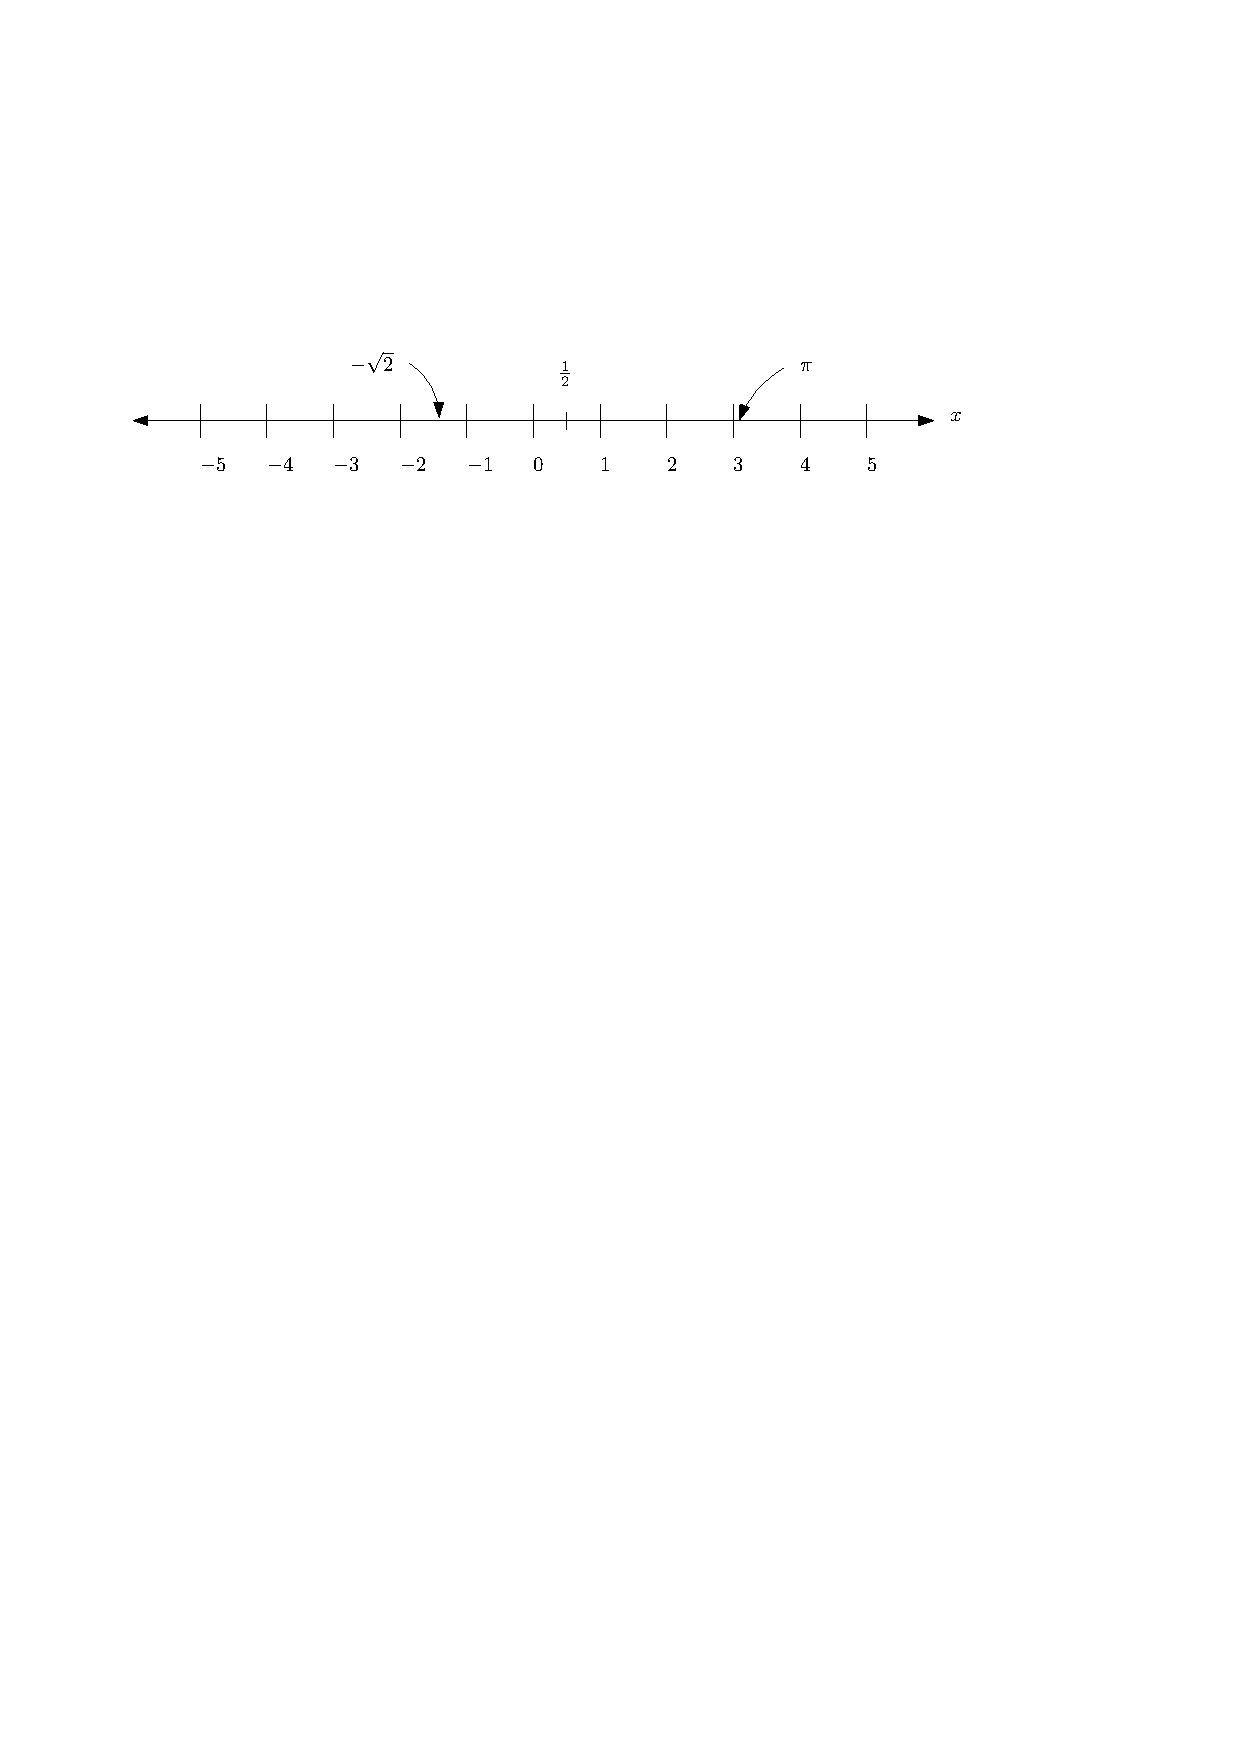
\includegraphics[scale=1]{graphics/number-line.pdf}
\end{center}

\subsubsection*{Complex numbers as extension of reals}

Continuing the pattern of the basic number system we can ask what are solutions of equations of the form $x^2+a = 0$ or $x^2 + 2ax +a^2 + b^2 = 0$ for $a,b \in \mathbb{R}$ ? As above, finding such solutions requires moving to a larger set of numbers, the \emph{complex numbers} denoted $\mathbb{C}$.

A complex variable $z\in\mathbb{C}$ can be written as $z = a + j\, b$ for $a,b\in\mathbb{R}$, where $j$ is the imaginary unit and $j^2 = -1$. Note in mathematics the imaginary unit is denoted $i$; this difference is purely historical. Some basic definitions:

\begin{itemize}
\item the \emph{real part} $\Re(z) = \text{Re}(z) = a$
\item the \emph{imaginary part} $\Im(z) = \text{Im}(z) = b$
\item two complex numbers $z_1, z_2\in \mathbb{C}$ are equal if $\text{Re}(z_1) = \text{Re}(z_2)$ and $\text{Im}(z_1) = \text{Im}(z_2)$
\item $\mathbb{R} \subset \mathbb{C}$, when $b = 0$ and we say that the number is purely real
\item if $a = 0$ we say the number is purely imaginary
\item the \emph{complex conjugate} of $z = a + jb$ is $z^* = a - jb$.
\end{itemize}

\subsubsection*{Operations on complex numbers}

Arithmetic operations on complex numbers are defined using the algebra of real numbers, replacing $j^2 = -1$. Given complex numbers $a + j\, b$ and $c + j\, d$

\begin{description}
\item[addition] $(a + jb) + (c +jd) = (a+c) + j(b+d)$
\item[subtraction] $(a + jb) - (c +jd) = (a-c) + j(b-d)$
\item[multiplication] $(a + jb)\cdot(c +jd) = ac + jbc + jad + j^2 bd = (ac-bd) + j(bc+ad)$
\item[division] $\frac{(a + jb)}{(c +jd)} = \frac{ac+jbc-jad-j^2 bd}{c^2 -j^2 d^2} = \frac{(ac+bd) + j(bc-ad)}{c^2 + d^2} = \frac{ac+bd}{c^2 + d^2} + j \frac{bc-ad}{c^2 + d^2}$
\end{description}


\subsubsection*{Basic properties of complex numbers}

Let $z_1, z_2, z_3 \in \mathbb{C}$, then:

\begin{description}
\item[closure property] $z_1 + z_2 \in \mathbb{C}$ and  $z_1 \cdot z_2 \in \mathbb{C}$ 
\item[communative property] $z_1 + z_2 = z_2 + z_1$ and $z_1 \cdot z_2 = z_2 \cdot z_1$ 
\item[associative property] $z_1 + (z_2 + z_3) = (z_1 + z_2) + z_3$ and $z_1 \cdot (z_2 \cdot z_3) = (z_1 \cdot z_2) \cdot z_3$ 
\item[identity elements] $0 = (0 + j0) \in \mathbb{C}$ is the identity element for addition since $z_1 + 0 = z_1$ and $1 = 1 + j0 \in \mathbb{C}$ is the identity element for multiplication since $z_1\cdot 1 = z_1$ 
\item[inverse elements] for any $z_1$ there exists an inverse $z_2 = -z_1$ such that $z_1 + z_2 = 0$, and for any $z_1 \neq 0$ there exists an inverse $z_2 = z_1^{-1} = \tfrac{1}{z_1}$ such that $z_1 \cdot z_2 = 1$
\end{description}

\subsubsection*{Absolute Value (Magnitude) of complex numbers}

The absolute value or \textit{magnitude} of a complex number $z = a + jb$ is denoted $|z| = |a+jb|$ and is given by
\[
|a + jb| = \sqrt{a*2 + b^2}
\]
For complex numbers $z_1, z_2, \ldots, z_n$, the following useful properties hold
\begin{itemize}
\item $|z_1\cdot z_2 \cdots z_N| = |a_1|\cdot |z_2|\cdots|z_N|$
\item $\left| \frac{z_1}{z_2}\right| = \frac{|z_1|}{|z_2|}$ for $z_2 \neq 0$
\end{itemize}

\subsubsection*{Argument (Angle) of complex numbers}
The argument or \textit{angle} of a complex number $z = a + jb$ is denoted $\angle z = \angle(a+jb)$ and is given by
\[
\angle(a + jb) = \arctan\frac{b}{a}
\]
Take care when computing this number on your calculator (or in a programming language) so that it produces and angle in radians and in the correct quadrant. For example $\angle(-1-j1) = \arctan\frac{-1}{-1} = \frac{5\pi}{4} = -\frac{3\pi}{4}$ is different from $\angle(-1-j1) = \arctan\frac{-1}{-1} = \arctan\frac{1}{1} = \frac{\pi}{4}$, the later being incorrect.

\subsubsection*{Cartesian and Polar representation of complex numbers}

A complex number $z$ can be represented in Cartesian form as a pair of numbers in the \textit{Complex Plane}, $(\Re{z},\Im{z})$. The same $z$ can be represented in polar form as $z = |z|\cdot e^{j\angle z}$. We can convert between the representations using  $\Re{z} = |z| \cos(\angle z)$ and $\Im{z} = |z| \sin(\angle z)$. The following relations hold

\begin{itemize}
\item Multiplication by $j$ is equivalent to rotation by $\tfrac{\pi}{2}$
\[
j\cdot z = e^{j\tfrac{\pi}{2}}\cdot |z|\cdot e^{j\angle z} = |z|\cdot e^{j(\angle z + \tfrac{\pi}{2})} 
\]
\item Division by $j$ is equivalent to rotation by $- \tfrac{\pi}{2}$
\[
\frac{1}{j}\cdot z = e^{-j\tfrac{\pi}{2}}\cdot |z|\cdot e^{j\angle z} = |z|\cdot e^{j(\angle z - \tfrac{\pi}{2})} 
\]
\end{itemize}

A related expression that will be very useful to us is \textit{Eulers formula}: $e^{j\theta} = \cos(\theta) + j\sin(\theta)$. From this we can derive the relations:
\[
\cos(\theta) = \frac{1}{2} e^{j\theta} + \frac{1}{2} e^{-j\theta} 
\]
\[
\sin(\theta) = \frac{1}{2j} e^{j\theta} - \frac{1}{2j} e^{-j\theta} 
\]

These representations and relations can be visualized as follows
\begin{center}
  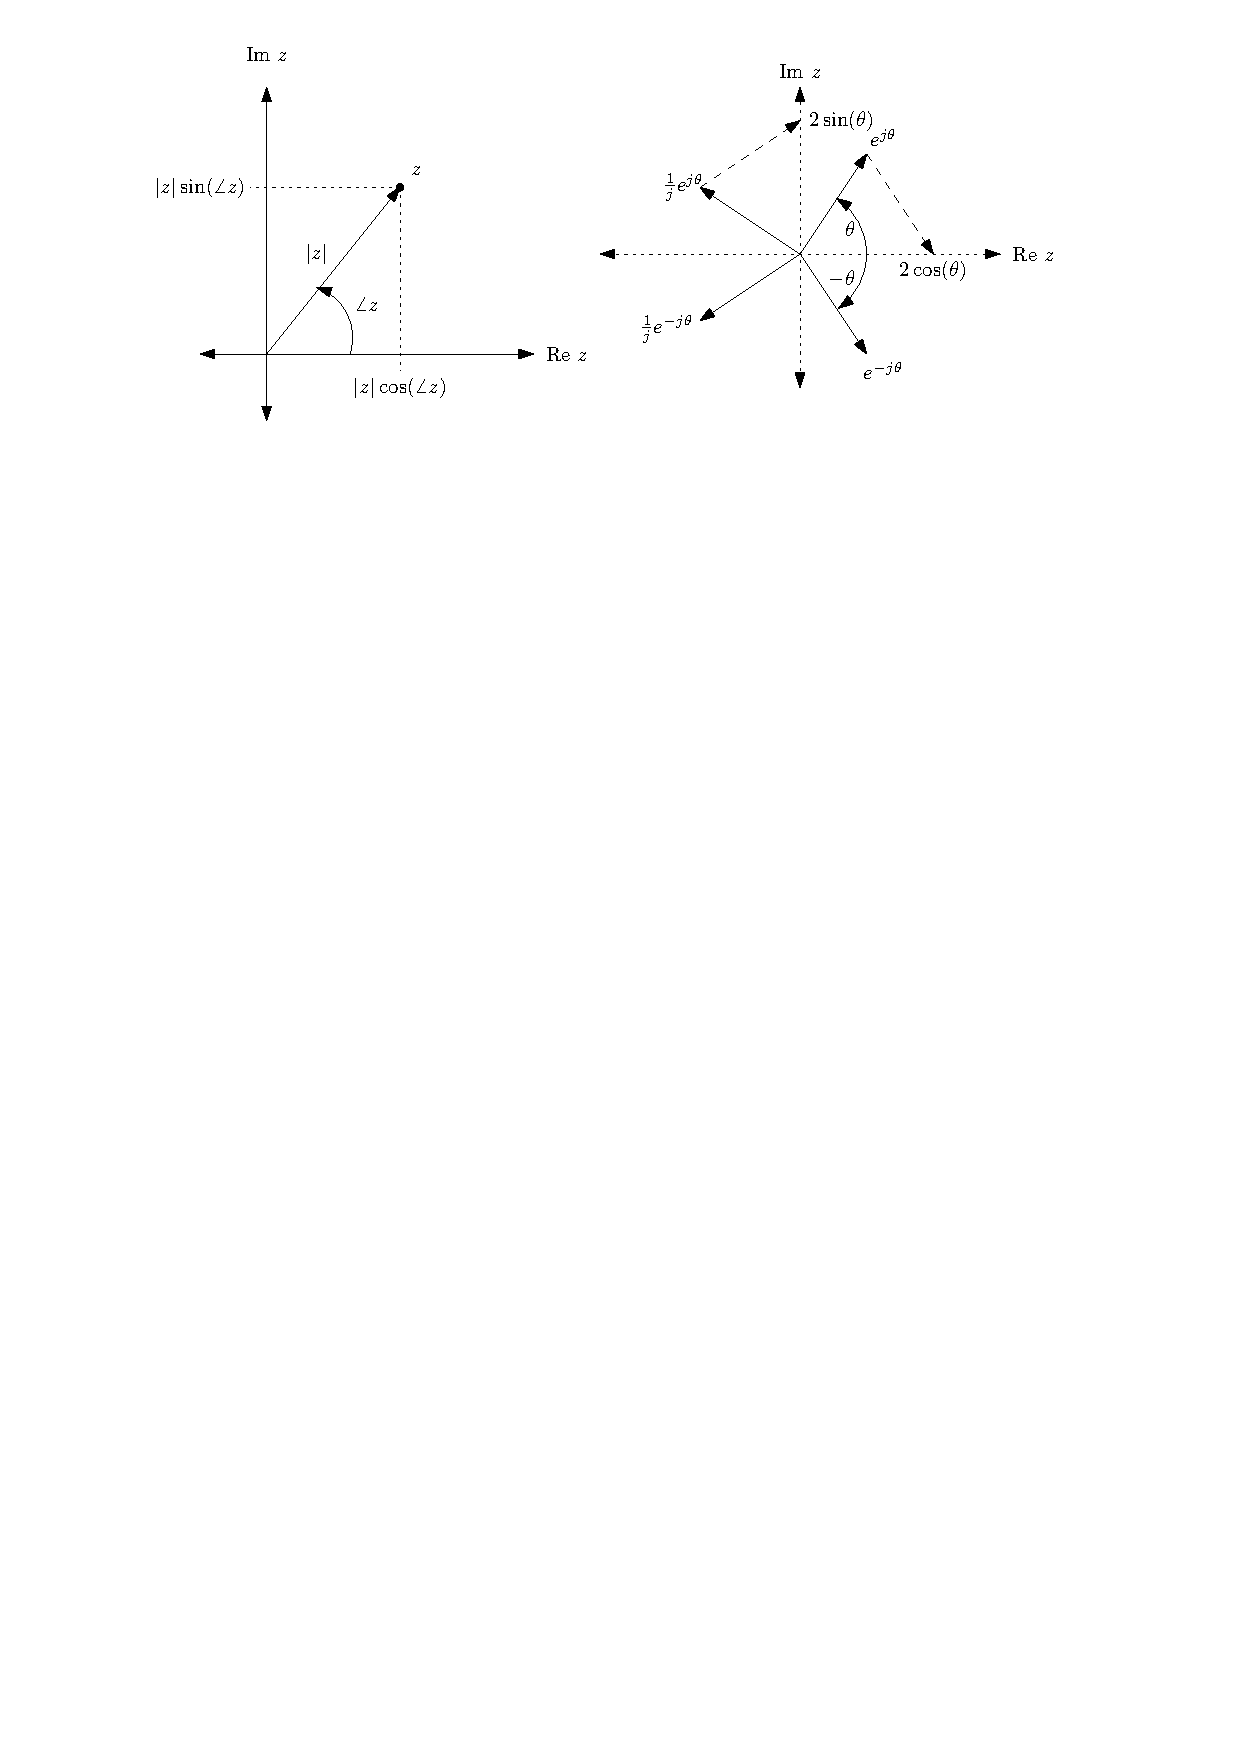
\includegraphics[scale=1]{graphics/complex-viz-prereq.pdf}
\end{center}

\subsubsection*{Complex numbers as roots of polynomial equations}

Recall our original motivation for complex numbers, as solutions to polynomials. Consider the $N^\text{th}$ order polynomial
\[
z^N + a_N z^{N-1} + \cdots + a_2 z + a_1 
\]
where in cases of interest to us in this course the $N$ coefficients $a_{N}, \cdots, a_1$ are real. In such cases the polynomial can be factored into
\[
z^N + a_{N} z^{N-1} + \cdots + a_2 z + a_1 = (z-z_1)\cdot(z-z_2)\cdots(z-z_N)
\]
where the $z_i$ are the $N$ \textit{roots} of the polynomial. These are complex numbers in general with two cases:

\begin{itemize}
\item the root is real
\item the root is complex or purely imaginary, in which case they come in congugate pairs 
\end{itemize}

Note: the \texttt{roots} function in Matlab can be used to find the roots of any order polynomial given a vector of coefficients.

\subsection{Calculus}

Calculus is used heavily in the course. Here we remind ourselves of some basic facts. Consult your calculus text for more details.

\subsubsection*{Functions}

A function is a mapping between sets
\[
f: A \rightarrow B
\]
where $A$ is a set called the {\it domain} and $B$ is a set called the {\it co-domain}. In this course we are primarily concerned with four kinds of functions

\begin{itemize}
\item the real-valued functions of an integer variable $f:\mathbb{Z}\mapsto\mathbb{R}$
\item the complex-valued functions of an integer variable $f:\mathbb{R}\mapsto\mathbb{C}$
\item the real-valued functions of a real variable $f:\mathbb{R}\mapsto\mathbb{R}$
\item the complex-valued functions of a real variable $f:\mathbb{R}\mapsto\mathbb{C}$
\end{itemize}
We will also briefly discuss the the complex-valued functions of a complex variable $f:\mathbb{C}\mapsto\mathbb{C}$.

\subsubsection*{Visualizing Functions}

You are certainly familiar with the graph of functions $f:\mathbb{R}\mapsto\mathbb{R}$. To graph a complex-valued function of a single variable we need to plot two functions. Consider a function $z(t) \in \mathbb{C}$ for $t \in \mathbb{R}$ expressed in Cartesian form:
\[
z(t) = z_r(t) + j z_i(t) 
\]
where $z_r(t) = \Re(z(t))$ and $z_r(t) = \Im(z(t))$ are the real and imaginary parts of the complex value at a given $t$. We can plot these two real-valued functions to visualize the complex function. Similarly consider a function $z(t) \in \mathbb{C}$ for $t \in \mathbb{R}$ expressed in polar form:
\[
z(t) = z_m(t) e^{jz_a(t)}
\]
where $z_m(t) = |z(t)|$ and $z_a(t) = \angle z(t)$ are the magnitude and angle of the complex value at a given $t$. We can plot these two real-valued functions to visualize the complex function.

Another approach to visualizing a complex number is to plot it as the tip of a vector that moves as a function of the independent variable.

\begin{example} Consider the function $z(t) = e^{|t| + j2t}$. Lets convert it to polar and Cartesian form
  \begin{align*}
    z(t) &=  e^{|t| + j2t}\\
    &=  \underbrace{e^{|t|}}_{z_m(t)} e^{j\overbrace{2t}^{z_a(t)}}\\
    &=  e^{|t|} (\cos(2t) + j\sin(2t))\\
    &=  \underbrace{e^{|t|}\cos(2t)}_{z_r(t)} + j \underbrace{e^{|t|}\sin(2t)}_{z_i(t)}
  \end{align*}
  We can then visualize the function as plots of the real and imaginary functions,

  \begin{tabular}{cc}
  \begin{tikzpicture}
    \begin{axis}[xmin=-5, xmax=5, ymin = -1, ymax=1, samples=1000, xlabel=$t$, ylabel=$z_r(t)$]
      \addplot[blue, thick] (x,(cos(2*180*x/pi)*cos(2*180*x/pi)));
      \addplot[mark=none, black] coordinates {(0,-1) (0,1)};
      \addplot[mark=none, black] coordinates {(-5,0) (5,0)};
    \end{axis}
  \end{tikzpicture}
  &
  \begin{tikzpicture}
    \begin{axis}[xmin=-5, xmax=5, ymin = -10, ymax=10, samples=10, xlabel=$t$, ylabel=$z_i(t)$]
      \addplot[blue, thick] (x,2*x));
      \addplot[mark=none, black] coordinates {(0,-10) (0,10)};
      \addplot[mark=none, black] coordinates {(-5,0) (5,0)};
    \end{axis}
  \end{tikzpicture}
  \end{tabular}\\
  or the mangitude and angle functions,\\
  \begin{tabular}{cc}
  \begin{tikzpicture}
    \begin{axis}[xmin=-5, xmax=5, ymin = 0, ymax=1, samples=1000, xlabel=$t$, ylabel=$z_m(t)$]
      \addplot[blue, thick] (x,e^(-abs(x)));
      \addplot[mark=none, black] coordinates {(0,0) (0,1)};
      \addplot[mark=none, black] coordinates {(-5,1) (5,1)};
    \end{axis}
  \end{tikzpicture}
  &
  \begin{tikzpicture}
    \begin{axis}[xmin=-5, xmax=5, ymin = -10, ymax=10, samples=10, xlabel=$t$, ylabel=$z_a(t)$]
      \addplot[blue, thick] (x,2*x));
      \addplot[mark=none, black] coordinates {(0,-10) (0,10)};
      \addplot[mark=none, black] coordinates {(-5,0) (5,0)};
    \end{axis}
  \end{tikzpicture}
  \end{tabular}
\end{example}


\subsubsection*{Derivatives of real-valued functions}

For functions $f:\mathbb{R}\mapsto\mathbb{R}$ recall the derivative is the rate of change in the value as a function of the independent variable, and can be defined using a limit of a difference. Consider such a function $f(t)$ for $t\in\mathbb{R}$, it's derivative is given using a forward difference:

\[
\frac{df}{dt} (t) = \lim_{h->0} \frac{f(t+h)-f(t)}{h}
\]

Higher-order derivative are defined recursively. For example, the second derivative is

\[
\frac{d^2f}{dt^2} = \lim_{h->0} \frac{\frac{df}{dt}(t+h)-\frac{df}{dt}(t)}{h}
\]
In the general case the $N^\text{th}$ order derivative is
\[
\frac{d^Nf}{dt^N} = \lim_{h->0} \frac{\frac{d^{N-1}f}{dt^{N-1}}(t+h)-\frac{d^{N-1}f}{dt^{N-1}}(t)}{h}
\]

Note there are several different notations for derivatives, e.g. $\frac{df}{dt} = f^\prime (t) = \dot{f}(t)$, but we will use the former in most cases. We will also use the derivative operator notation $\frac{d^Nf}{dt^N} = (D^N f)(t)$, which is convenient for higher-order derivatives.

A function with finite derivatives for all values of the independent variable is called \textit{continuous}. Values of the independent variable where the derivative is not finite are called \textit{discontinuities}. A function with a finite number of discontinuities is called \textit{piecewise continuous}.

\subsubsection*{Integrals of real-valued functions}

\subsection{Differential Equations}

This course assumes a background in basic differential equations. However, we use only consider linear, constant-coefficient differential equations.

\subsubsection*{linear, constant-coefficient differential equations, homogeneous and particular solutions}

Recall,

\subsection{Circuits}

ECE 2024 is required for knowledge of continuous signals representation as voltages and currents, and the analysis and construction of circuits containing resistors, capacitors, inductors, and operational amplifiers.

\begin{itemize}
\item $v = iR$\hspace{2em}
  \begin{circuitikz}[american voltages,scale=0.8, every node/.style={transform shape}]
    \draw
    (0,0) to[R,l=$R$] (4,0);
  \end{circuitikz}
  
\item $i = Cv^\prime$ \hspace{2em}
  \begin{circuitikz}[american voltages,scale=0.8, every node/.style={transform shape}]
    \draw
    (0,0) to[C,l=$C$] (4,0);
  \end{circuitikz}
\item $v = Li^\prime$ \hspace{2em}
  \begin{circuitikz}[american voltages,scale=0.8, every node/.style={transform shape}]
    \draw
    (0,0) to[L,l=$L$] (4,0);
  \end{circuitikz}
\item KVL
\item KCL
\item Ideal Op-Amp
\end{itemize}

\subsubsection*{KVL}

\subsubsection*{KCL}

\subsubsection*{Ideal OpAmps}

\subsubsection*{from circuit to differential equation}

\subsubsection*{using LiaB and building/measuring circuits}

\subsection{Programming}

ECE 2514 is required for the ability to model and simulate physical systems using computational tools, and basic programming ability.

\begin{itemize}
\item Matlab for general computation and plotting
\item C++ (a small subset) for implementing digital filters
\end{itemize}

\subsubsection*{plotting and vizualization with Matlab/Python/Julia}

\subsubsection*{Computation with C or C++}

\subsection{Digitial Systems}

ECE 2544 is required for for knowledge of digital signal representation and the analysis and construction of circuits containing combinatorial and sequential logic.

\subsubsection*{binary representation of integers vs floating point}

\subsubsection*{shift registers}

\subsubsection*{adders and multipliers}
